\chapter{Intensity transmission optimization}

The previous two chapters addressed the characteristics of the \gls{rf}
signal and the intensity transmission of the \gls{aod}. Therewith the
groundwork has been set out to finally approach the mission of minimizing the
intensity variance to obtain a homogenous optical potential.

But how do we minimize the intensity variance? The \gls{dds} permits to read
$N=1024$ amplitude values from memory. The optimization problem therefore is to
minimize the variance of the intensity distribution $I(A)$ subject to an
amplitude vector $A\in[0,1]^N$. The conclusions drawn from the intensity
measurements suggest that we have to expect non-linear, irregular behaviour
in $I(A)$. and indeed first attempts to model $I(A)$ through polynomial fits,
multilayer perceptron networks and least-squared minimizations have failed.

During these optimization procedures we observed that changing an amplitude
value $A_i\in A$ does affect the intensity voltage at subsequent
$A_{i+1},\dots,A_N$. Fortunately we found that by respecting the amplitude
order with respect to increasing frequency during optimization we where able
to bypass these effects. Further we created amplitude segments
$\left(A_j,\dots,A_{j+m}\right)$ consisting of $m$ ordered amplitude values
to reduce the optimization time. Optimization then was performed through
random search which was proven to yield better results as grid search
\cite{Bergstra2012}.

\subsubsection{Overview}

First, we want to provide an overview of the final optimization results
obtained at different hyperparameters for the random search. The
hyperparameter includes the number of amplitude segments $N/m$ and the target
intensity.
\begin{figure}[ht]
  \centering
  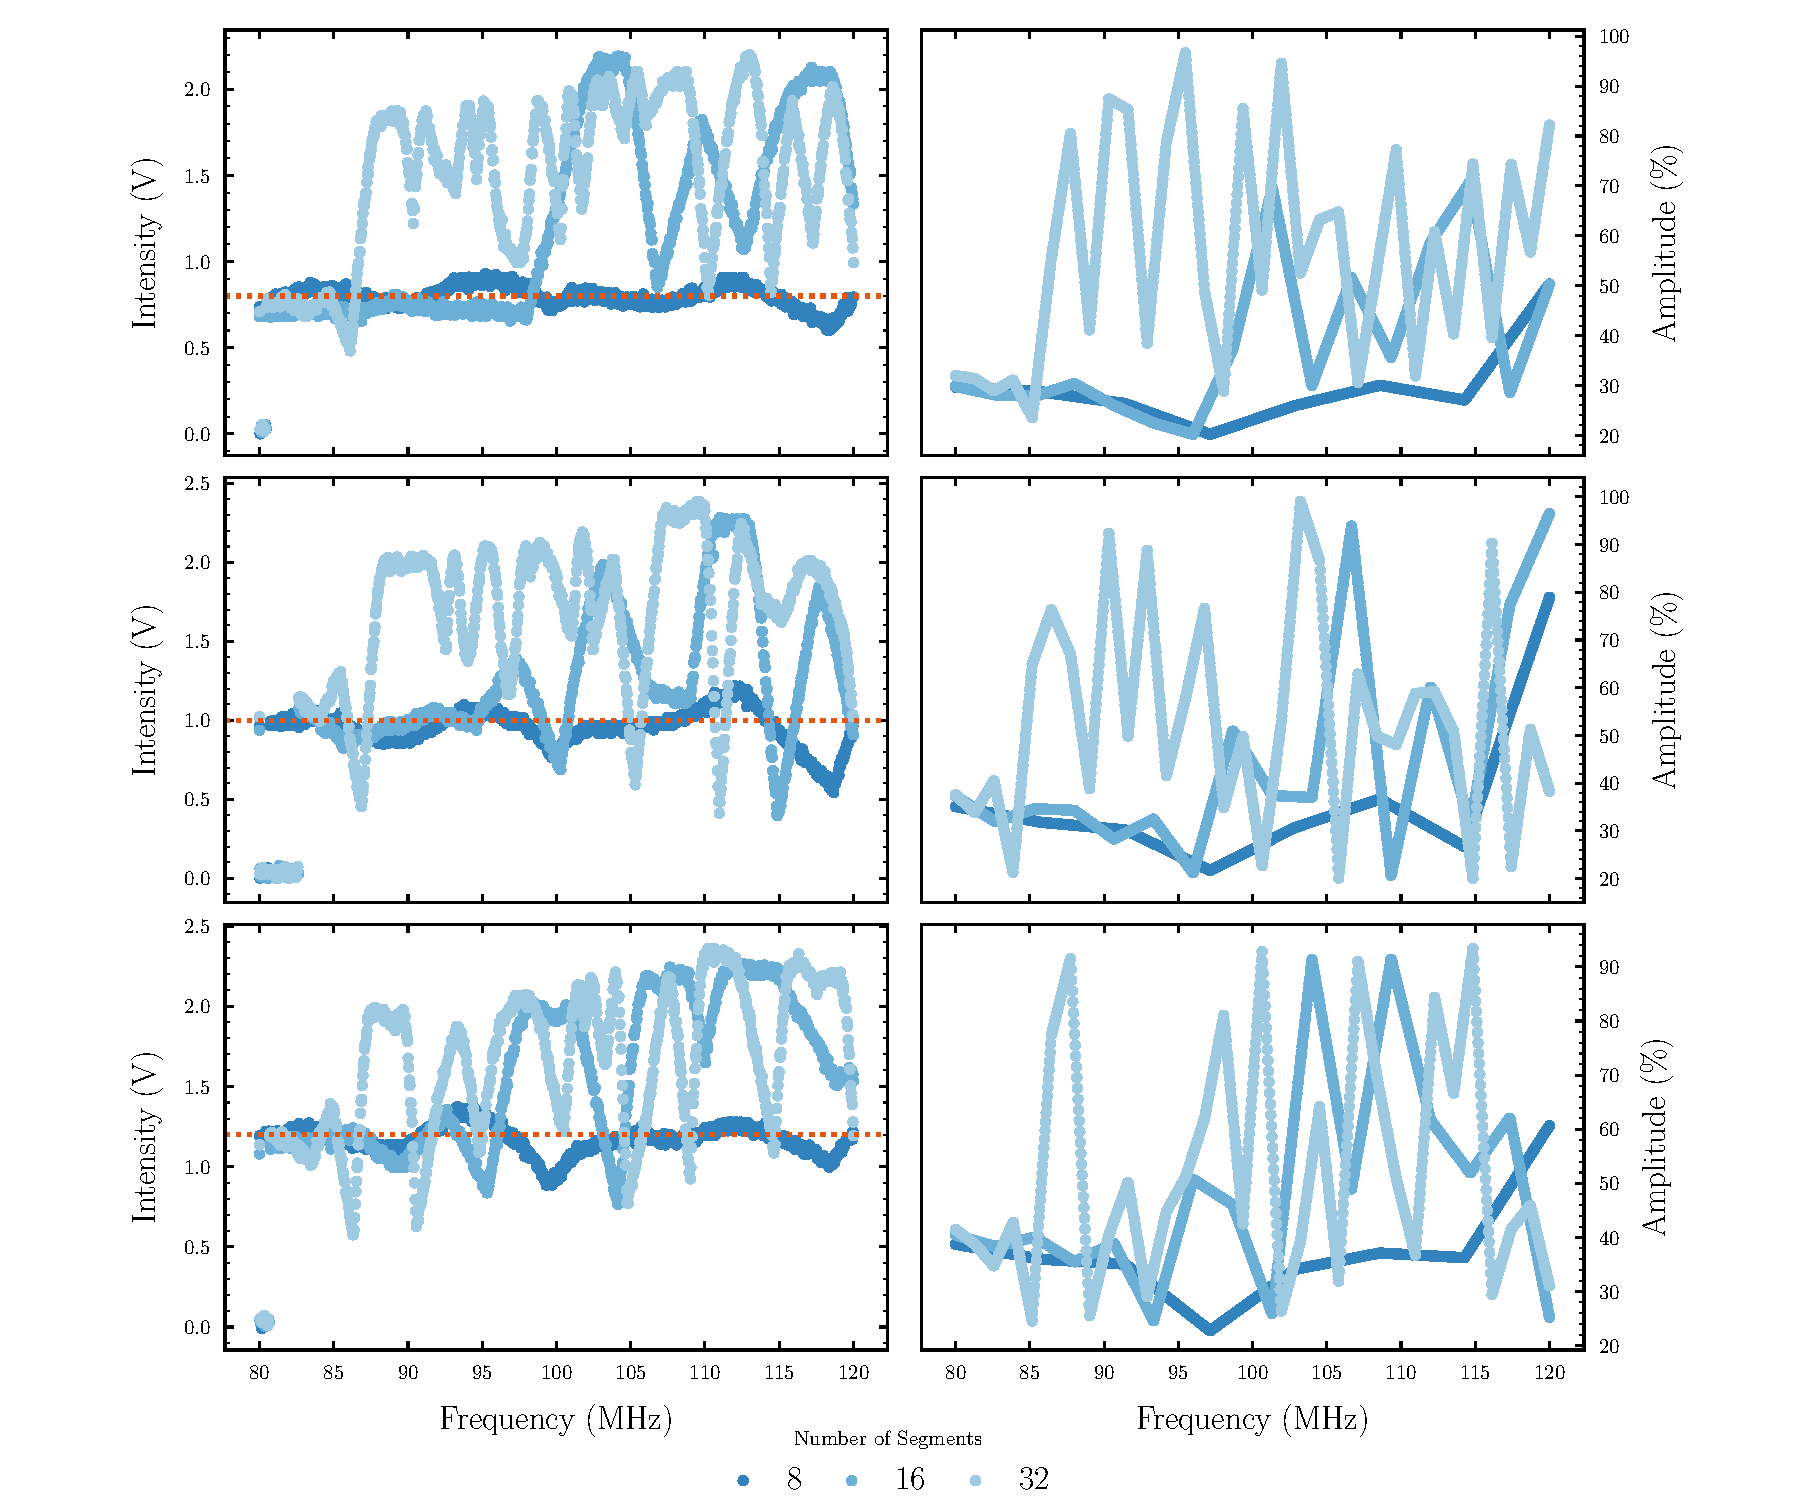
\includegraphics[width=\textwidth]{\figuredir{intensity/optimization/overview.pdf}}
  \captionsetup{width=.8\textwidth}
  \caption{Minimized intensity variance for different target intensities
  and number of amplitude segments. We note heavy oscillations for
  amplitude segments greater than eight.}
  \label{fig:intensity_optimization_overview}
\end{figure}
In \Cref{fig:intensity_optimization_overview} we present the final
optimization results for target intensities of \SI{800}{\milli\volt},
\SI{1000}{\milli\volt} and \SI{1200}{\milli\volt} and amplitude segments
$8,16,32$. We observe heavy oscillations for amplitude segments greater than
eight. The optimization results using 16 amplitude segments performs better
than the run with 32 amplitude segments.

We assume that inductive effects occur when choosing more amplitude segments
that consolidate a non-linear intensity response. For the sake of simplicity
we will first limit us to the case of eight amplitude segments.

\begin{figure}[ht]
  \centering
  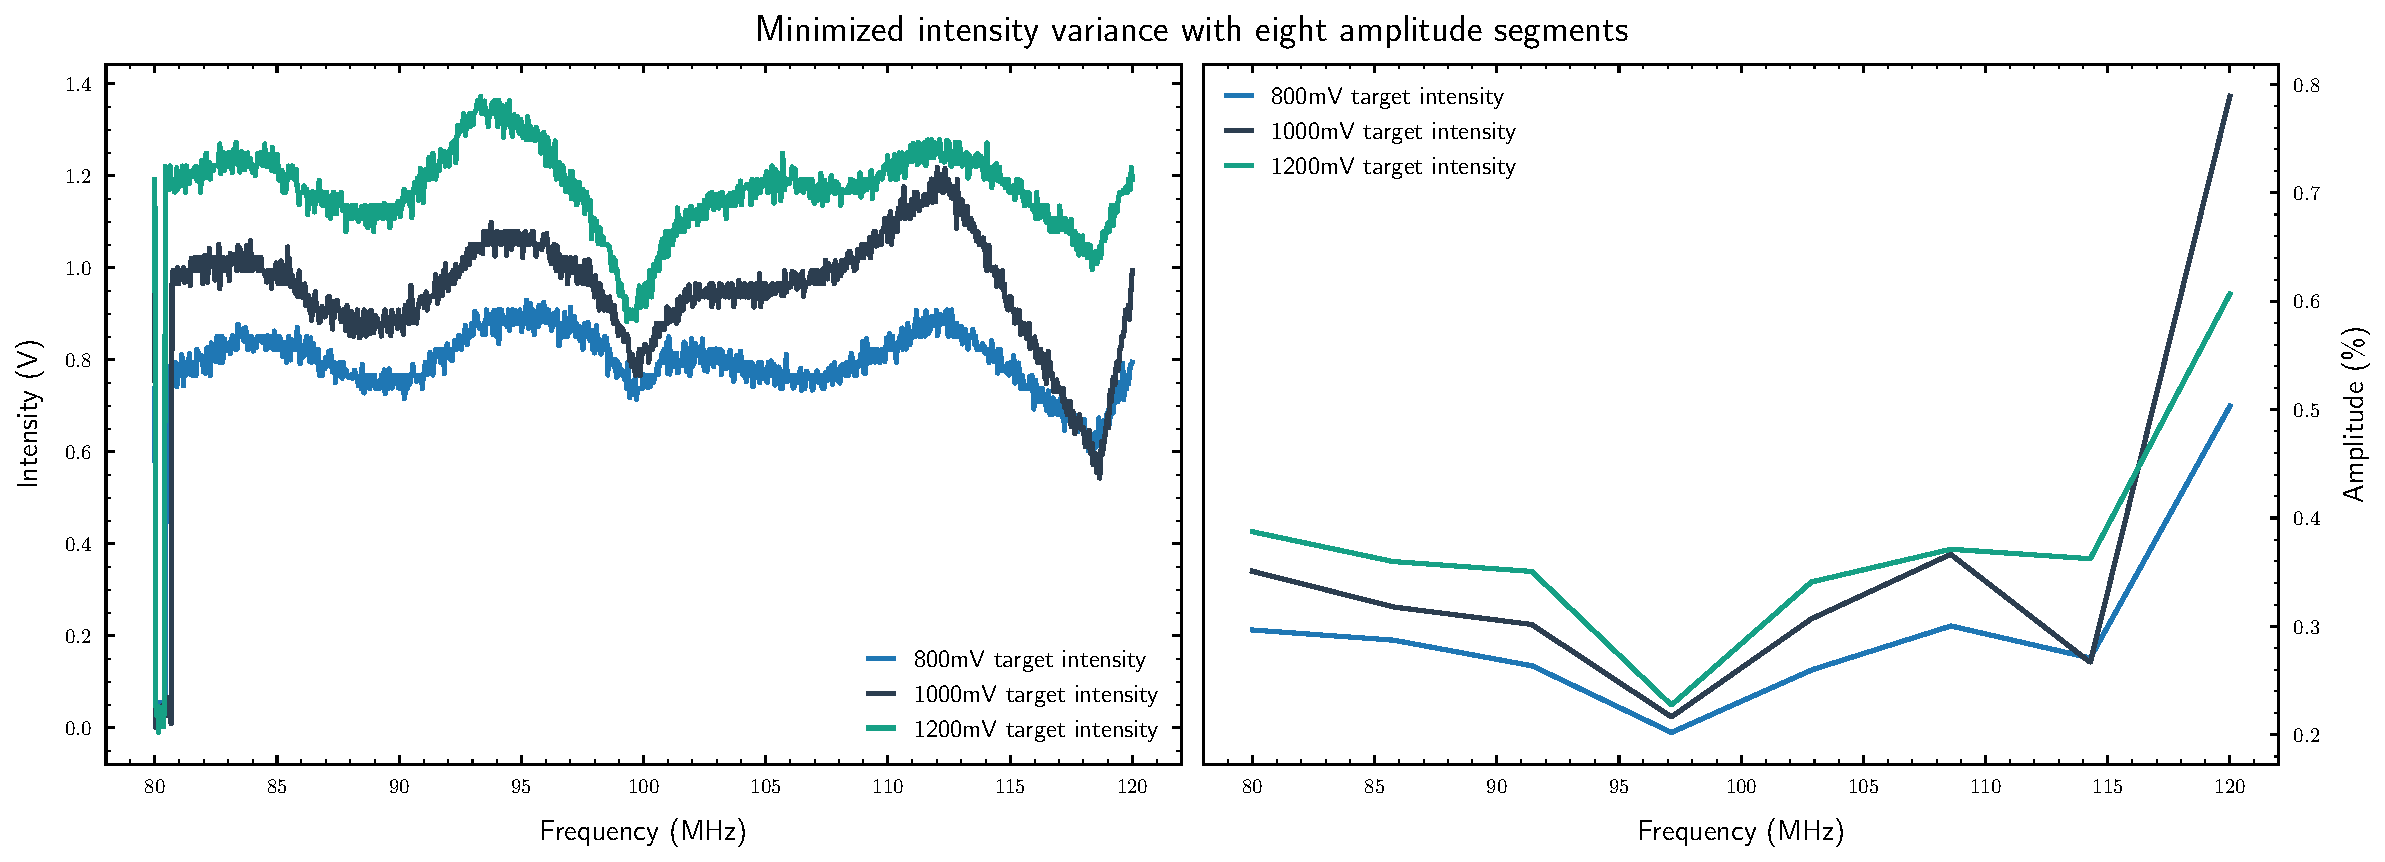
\includegraphics[width=\textwidth]{\figuredir{intensity/optimization/intensity-amplitude.pdf}}
  \captionsetup{width=.8\textwidth}
  \caption{Final result of the intensity variance minimization and the
  corresponding amplitude segment values obtained through random search with
  eight independent amplitude segments.}
  \label{fig:intensity_optimization_intensity_amplitude}
\end{figure}

In \Cref{fig:intensity_optimization_intensity_amplitude} we have a closer
view on the first column of \Cref{fig:intensity_optimization_overview}. We
can notice similar characteristics observed in the \gls{rf} signal. In
particular the more power drop near the center frequency is present and the
linear power fall off with the frequency in the second half of the frequency
sweep.

\subsubsection{Process}

We now want to elaborate on the optimization process. We limit ourselves to
the optimization process with eight amplitude segments as it was the most
successful one and can be covered completly with eight plots.

\begin{figure}[ht]
  \centering
  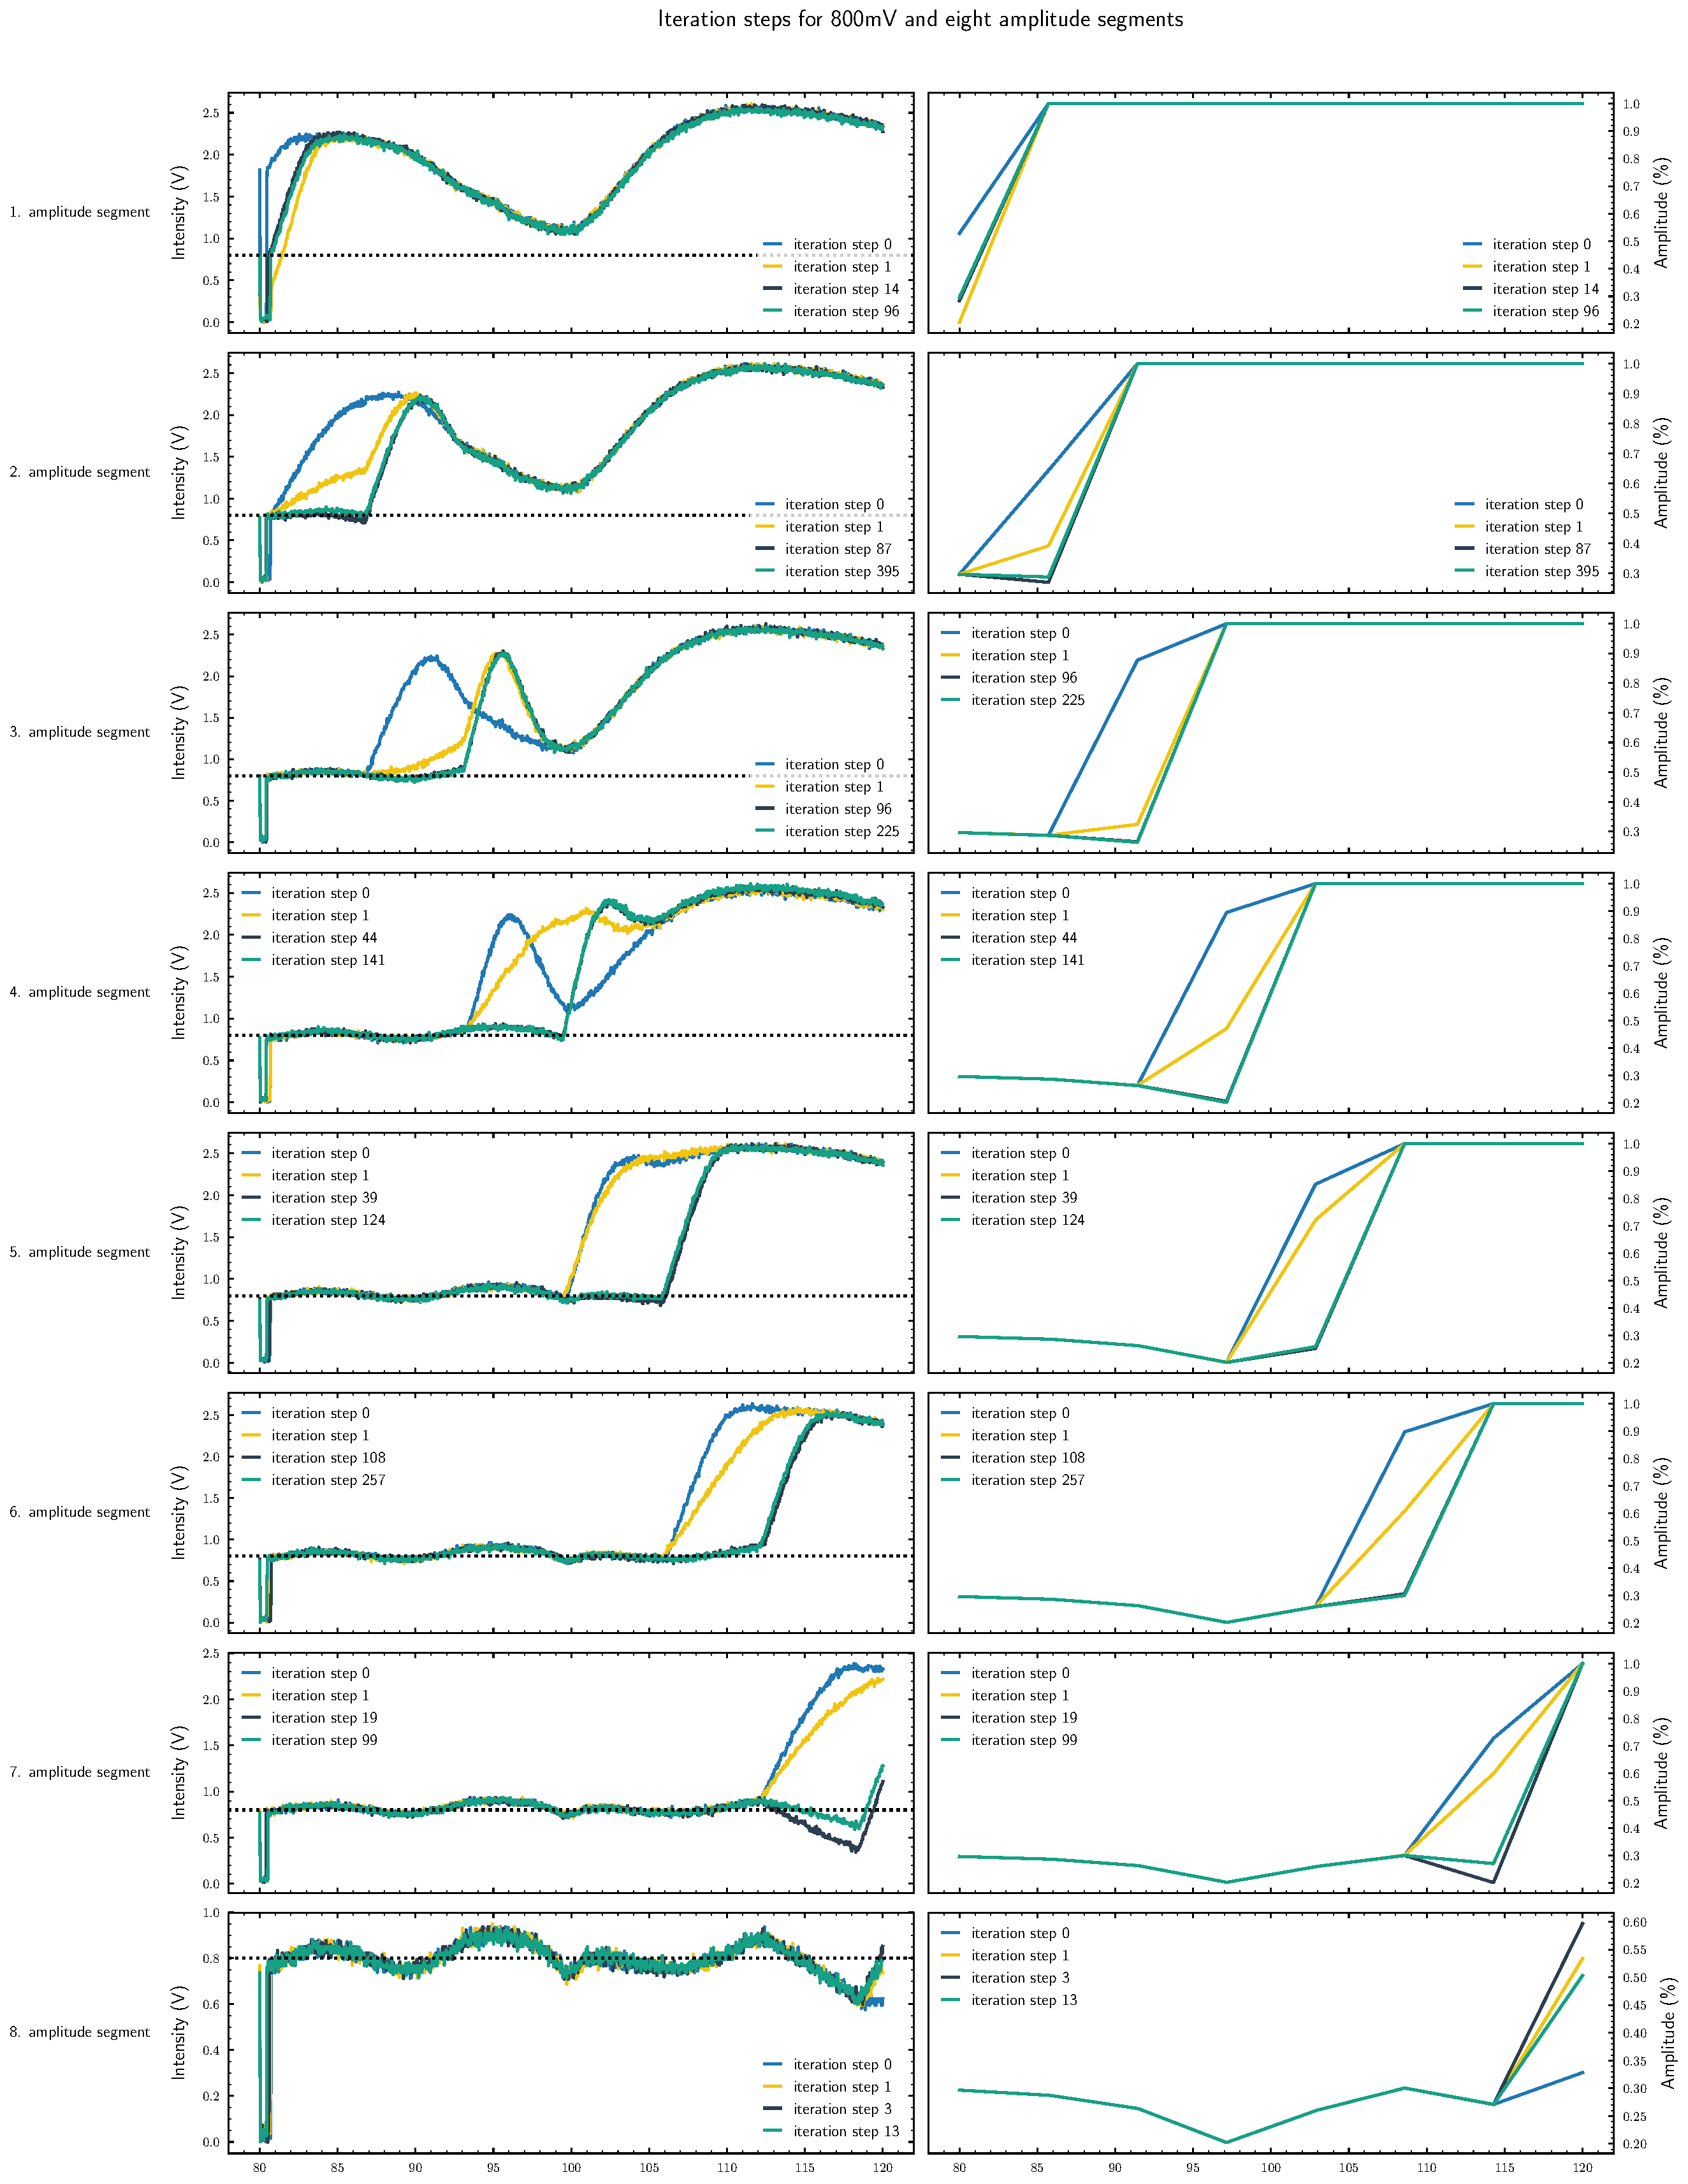
\includegraphics[width=\textwidth]{\figuredir{intensity/optimization/process.pdf}}
  \captionsetup{width=.8\textwidth}
  \caption{Intensity and amplitude at different stages of the optimization
  process. In each column a different amplitude segment is optimized.
  The different traces in each plot mark the respective iteration.}
  \label{fig:intensity_optimization_process}
\end{figure}

In \Cref{fig:intensity_optimization_process} we see the intensity and
amplitude at different optimization stages. At each stage one amplitude
segment is sampled from a uniform distribution over $[.2, .8]$. The intensity
segment associated with this amplitude segment is then used to calculate
the \gls{mse} and compare it to the previous best \gls{mse}. If the new
\gls{mse} is less than the previous best \gls{mse} the previous best \gls{mse}
is updated and the amplitude segment value is saved. This procedure is
repeated 500 times. Every time a new best value was found we saved the
data. For the diagrams we choose the four most separated iteration steps to
visualize the process of the optimization.

If we take a look at the succeeding segment from the currently optimized
amplitude segment we observe that these differ for different amplitude
values and henceforth confirms that amplitude values are not independent but
affect subsequent segments.

\subsubsection{Failure}

With the optimization showing reasonable convergence for eight amplitude
segments we would expect it to improve if we choose a more amplitude segments,
yet we observed heavy oscillations. In this section we want to check the
optimization process in the case of 32 amplitude segments to investigate in
possible origins of the optimization failure.

\begin{figure}[ht]
  \centering
  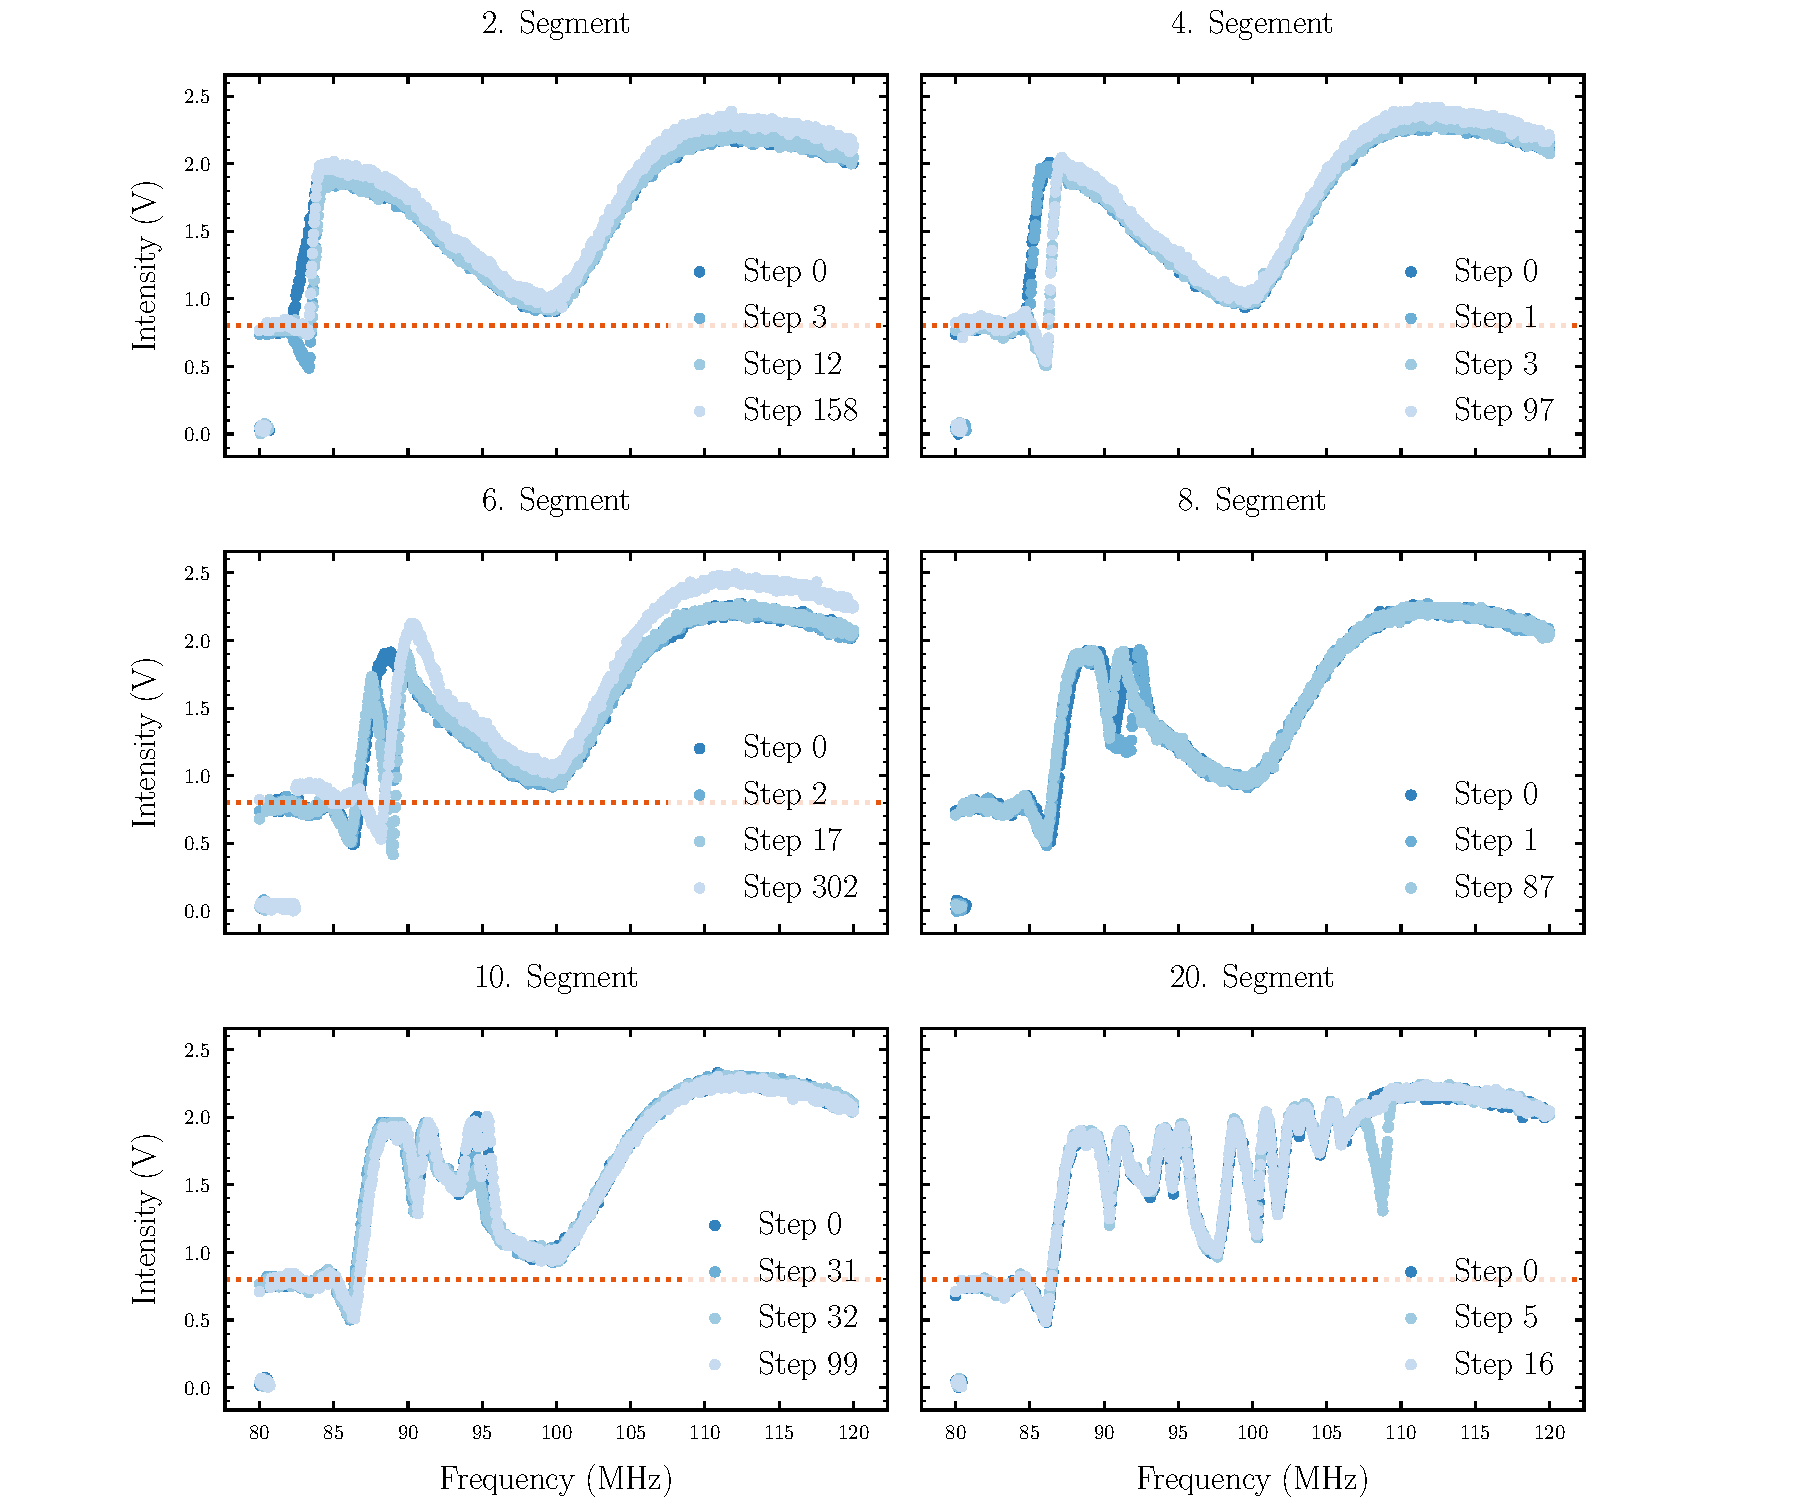
\includegraphics[width=\textwidth]{\figuredir{intensity/optimization/failure.pdf}}
  \captionsetup{width=.8\textwidth}
  \caption{Optimization progress for the 2.,4.,6.,8.,10. and 20. amplitude
  segment of the failed optimization run with 32 amplitude segments. We can
  see that with increasing amplitude segments the non-linear response
  following the optimized amplitude segment increases.}
  \label{fig:intensity_optimization_failure}
\end{figure}

In \Cref{fig:intensity_optimization_failure} we can see the optimization
progress for selected amplitude segments of the optimization run with 32
segments. We observe that with the non-linear response following the actual
optimized amplitude segment increases more and more.

\subsubsection{Summary}

Our attemps to minimize the intensity variance where of mixed success. One
the one hand side we were able to minimize the intensity deviation down
to \SI{100}{\milli\volt} on the other hand we were not able to train any
model on the intensity response that would allow fast optimization or even
predicition of the expected intensity response given an amplitude
configuration.

However we also found out that irregularities arise with increase in the
number of amplitude segments. We suspect that fast changes of the output
amplitude draws power that may non deterministicyl affect the next clock
cycle inside the \gls{dds}. Given that the one dimensional optimizations
already required multiple hours to run and the non-linear response between
amplitude segments we do not believe that it is not in the capabilites of the
\gls{dds} to compensate for the two dimensional intensity distribution
measured in the previous chapter.
